\documentclass{article}
\usepackage{graphicx} % Required for inserting images
\usepackage{amsmath}  % Required for align environment
\usepackage[margin=1in]{geometry}


\title{ELCT 432 Assignment \#2}
\author{Jacob C. Vaught}
\date{September 6th 2023}

\begin{document}
\maketitle

\newpage
\section*{Problem \#1}
To calculate the power of a signal \(x(t)\), the formula for continuous-time signals is
\[
P = \lim_{{T \to \infty}} \frac{1}{T} \int_{{-T/2}}^{{T/2}} |x(t)|^2 \, dt
\]

\subsection*{Part a: \( x(t) = \sin(4000 \pi t) \)}

The power is calculated as follows:
\[
\begin{aligned}
P &= \lim_{{T \to \infty}} \frac{1}{T} \int_{{-T/2}}^{{T/2}} |\sin(4000 \pi t)|^2 \, dt \\
&= \lim_{{T \to \infty}} \frac{1}{T} \int_{{-T/2}}^{{T/2}} \sin^2(4000 \pi t) \, dt \\
&= \lim_{{T \to \infty}} \frac{1}{T} \int_{{-T/2}}^{{T/2}} \frac{1 - \cos(8000 \pi t)}{2} \, dt \\
&= \frac{1}{2} \lim_{{T \to \infty}} \frac{1}{T} \left[ T - \frac{\sin(8000 \pi t)}{8000 \pi} \Bigg|_{{-T/2}}^{{T/2}} \right] \\
&= \frac{1}{2}
\end{aligned}
\]

\subsection*{Part b: \( x(t) = 2 \cos(11000 \pi t) \)}

\[
\begin{aligned}
P &= \lim_{{T \to \infty}} \frac{1}{T} \int_{{-T/2}}^{{T/2}} |2 \cos(11000 \pi t)|^2 \, dt \\
&= \lim_{{T \to \infty}} \frac{1}{T} \int_{{-T/2}}^{{T/2}} 4 \cos^2(11000 \pi t) \, dt \\
&= \lim_{{T \to \infty}} \frac{1}{T} \int_{{-T/2}}^{{T/2}} 2 + 2 \cos(22000 \pi t) \, dt \\
&= 2 \lim_{{T \to \infty}} \frac{1}{T} \left[ T + \frac{\sin(22000 \pi t)}{22000 \pi} \Bigg|_{{-T/2}}^{{T/2}} \right] \\
&= 2
\end{aligned}
\]

\subsection*{Part c: \( x(t) = \sin(4000 \pi t) + 2 \cos(11000 \pi t) \)}

\[
\begin{aligned}
P &= \lim_{{T \to \infty}} \frac{1}{T} \int_{{-T/2}}^{{T/2}} |\sin(4000 \pi t) + 2 \cos(11000 \pi t)|^2 \, dt \\
&= \lim_{{T \to \infty}} \frac{1}{T} \int_{{-T/2}}^{{T/2}} \sin^2(4000 \pi t) + 4 \cos^2(11000 \pi t) + 4 \sin(4000 \pi t) \cos(11000 \pi t) \, dt \\
&= P_{\text{first term}} + P_{\text{second term}} + P_{\text{cross term}} \\
&= \frac{1}{2} + 2 + 0 \\
&= \frac{5}{2}
\end{aligned}
\]

\newpage
\section*{Problem \#2}

\subsection*{What is the signal bandwidth?}

The baseband signal \( x(t) \) is defined to have a non-zero spectrum only for \( |f| < 1 \) MHz. Therefore, the bandwidth of the baseband signal is \( 2 \times 1 \) MHz = \( 2 \) MHz.

\subsection*{Sketching the Spectra}

\subsubsection*{Baseband Signal Spectrum \(X(f)\)}

For the baseband signal, the spectrum \( X(f) \) is non-zero only for \( |f| < 1 \) MHz. An arbitrary shape of \( X(f) \) is illustrated below.

\begin{figure}[h]
    \centering
    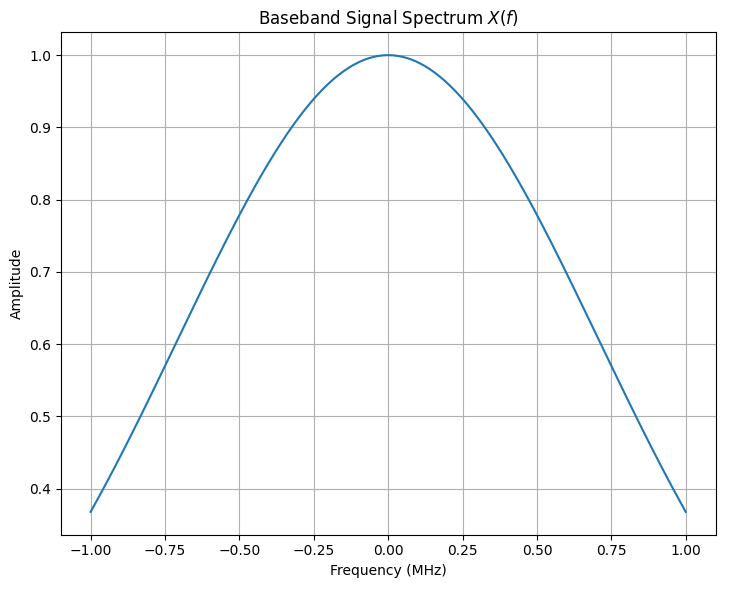
\includegraphics[width=1\textwidth]{baseband_signal.png}
    \caption{Sketch of the baseband signal spectrum \( X(f) \)}
\end{figure}
\newpage
\subsubsection*{Modulated Signal Spectrum \(Y(f)\)}

The modulated signal \( y(t) = e^{i 2 \pi f_c t} x(t) \) with \( f_c = 100 \) MHz will have a spectrum that is a shifted version of \( X(f) \). 

\begin{figure}[h]
    \centering
    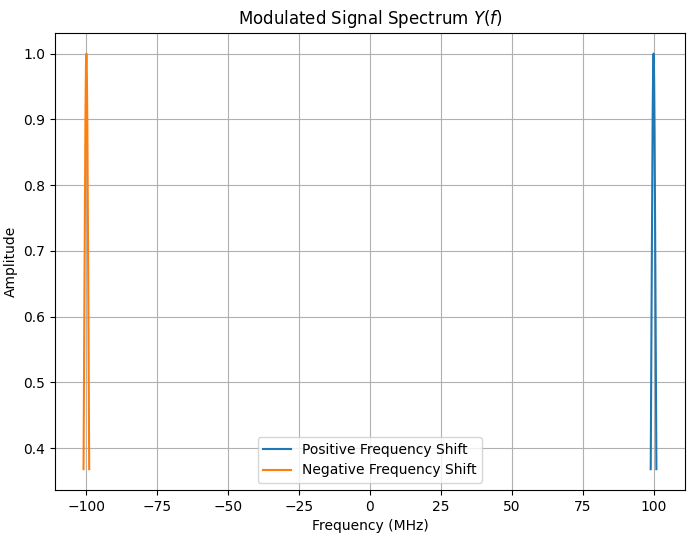
\includegraphics[width=1\textwidth]{modulated_signal.png}
    \caption{Sketch of the modulated signal spectrum \( Y(f) \)}
\end{figure}

The spectrum of \( y(t) \) will be centered at \( f = 100 \) MHz and will have the same shape as \( X(f) \), just shifted.

\newpage
\section*{Problem \#3}
\subsection*{Baseband Signal Spectrum \(F(f)\)}

The baseband signal has a spectrum \( F(f) \) with constant magnitude \( H_0 \) and bandwidth \( B \). 

\subsection*{Time-Domain Signal \(f(t)\)}

Due to the rectangular shape of \( F(f) \), the time-domain signal \( f(t) \) can be expressed as:

\[
f(t) = H_0 \cdot \text{sinc}\left(\frac{B}{2} \cdot t\right)
\]

\subsection*{Modulated Time-Domain Signal \(y(t)\)}

Upon modulation with a carrier frequency \( f_c \), the modulated signal \( y(t) \) becomes:

\[
y(t) = f(t) \cdot \cos(2\pi f_c t) = H_0 \cdot \text{sinc}\left(\frac{B}{2} \cdot t\right) \cdot \cos(2\pi f_c t)
\]
\newpage
\section*{Problem \#4}
\subsection*{In-Phase and Quadrature Components in Complex Lowpass Signal}

The complex lowpass signal, often denoted as $s(t)$, can be represented as:

\[
s(t) = I(t) \cos(2\pi f_0 t) - Q(t) \sin(2\pi f_0 t)
\]
Where:
\begin{itemize}
  \item $I(t)$ is the in-phase component
  \item $Q(t)$ is the quadrature component
  \item $f_0$ is the carrier frequency
\end{itemize}
The in-phase and quadrature components are crucial in practice because they allow the representation of both amplitude and phase information in the signal. This is particularly useful in modern communication systems for more efficient data transmission and signal processing.

\subsection*{Real Bandpass Signal from Complex Signals}

\subsubsection*{From Complex Bandpass Signal}

A real bandpass signal $x(t)$ can be obtained from a complex bandpass signal $s_{\text{BP}}(t)$ as follows:

\[
x(t) = \Re\{ s_{\text{BP}}(t) \}
\]

\subsubsection*{From Complex Lowpass Signal (Baseband Signal)}

A real bandpass signal $x(t)$ can also be obtained from a complex lowpass signal $s(t)$:

\[
x(t) = 2\Re\{ s(t) e^{j2\pi f_0 t} \}
\]

\subsection*{Fourier Transform Symmetry}

\subsubsection*{Real Bandpass Signal}

For a real signal $x(t)$, its Fourier Transform $X(f)$ will be symmetric, i.e., $X(f) = X^*(-f)$. This is a fundamental property of real signals.

\subsubsection*{Complex Bandpass Signal}

For a complex signal, assuming the imaginary part is non-zero, the Fourier Transform will not be symmetric. This is because a complex signal carries both magnitude and phase information, breaking the symmetry in its frequency domain representation.

\subsection*{Condition for Frequency Domain Symmetry in Complex Lowpass Signal}

A complex lowpass signal $s(t)$ will be symmetric in the frequency domain under the condition that it is conjugate symmetric in the time domain, i.e., $s(t) = s^*(-t)$.

\end{document}
